\section{Leading-Zero-Counter and Shifter (LZC) Compilation Example}
\label{sec:lzc}
In this section we provide a combined LZC and shifter DFiant implementation and describe its compilation process. We begin with a pseudo code\cite{muller2009handbook} as depicted in \fig{fig:LZC_pseudo_code}.
\begin{figure}[h]
\begin{algorithm}[H]
  \caption*{Combined leading-zero counting and shifting}
  \begin{algorithmic}
    \small
    \STATE{$k \leftarrow \left\lceil \log_2{n} \right\rceil$}
    \STATE{$x_k \leftarrow x$}
    
    \FOR{$i = k-1$ downto $0$}
    \IF{there are $2^i$ leading zeros in $x_{i+1}$} 
    \STATE{$d_i \leftarrow 1$}
    \STATE{$x_i \leftarrow x_{i+1}$, shifted left by $2^i$}
    \ELSE 
    \STATE{$d_i \leftarrow 0$}
    \STATE{$x_i \leftarrow x_{i+1}$}
    \ENDIF
    \ENDFOR
    \STATE{return $(d, x0)$}
  \end{algorithmic}
\end{algorithm}
\captionof{figure}{LZC and shifter pseudo code reference}
\label{fig:LZC_pseudo_code}
\end{figure}

The DFiant LZC and shifter implementation is very similar to the pseudo code reference, as can be seen in \fig{fig:LZC_DFiant_code}. This code is invoked internally by the FPMul implementation. 

\begin{figure}[h]
  \begin{minted}[autogobble,tabsize=2,frame=single,fontsize=\small]{Scala}
    def lzc_shift[N](num : DFBits[N]) = {
      val k = log2Up(num.width)
      val x = DFBits(num.width) := num
      val d = DFBits(k) := 0
      
      for (i <- k-1 downto 0) {
        ifdf (x.msbits(2~^i) == 0) {
          d(i) := 1
          x := x << 2~^i
        }
      }
      (d, x)
    }
  \end{minted}
  \captionof{figure}{LZC and shifter DFiant code}
  \label{fig:LZC_DFiant_code}
\end{figure}

When we apply \code{lzc\_shift} on an 8-bit vector \code{num}, the DFiant frontend compiler unrolls the \code{for} loop and converts the \code{ifdf} control statement into a mux. An equivalent unrolled code is given in \fig{fig:LZC_unrolled_code}. This code is close to the static single assignment (SSA) form intermediate representation (IR). The DFiant frontend IR is a dataflow graph as illustrated in \fig{fig:LZC_Dataflow}. The backend compiler converts the dataflow graph to Verilog and adds pipeline registers as required to achieve the target performance.

\begin{figure}[h]
  \begin{minted}[autogobble,tabsize=2,frame=single,fontsize=\small]{Scala}
  val x_3 = DFBits[8] := num
  val d_3 = DFBits[3] := 0
  val x_2 = mux(x_3.msbits(4)==0, x_3<<4, x_3)
  val d_2 = mux(x_3.msbits(4)==0, d_3(2):=1, d_3)
  val x_1 = mux(x_2.msbits(2)==0, x_2<<2, x_2)
  val d_1 = mux(x_2.msbits(2)==0, d_2(1):=1, d_2)
  val x_0 = mux(x_1.msbits(1)==0, x_1<<1, x_1)
  val d_0 = mux(x_1.msbits(1)==0, d_1(0):=1, d_1)
  return (d_0, x_0)
  \end{minted}
  \captionof{figure}{LZC and shifter unrolled DFiant code}
  \label{fig:LZC_unrolled_code}
\end{figure}


\begin{figure}[h]
  \centering
  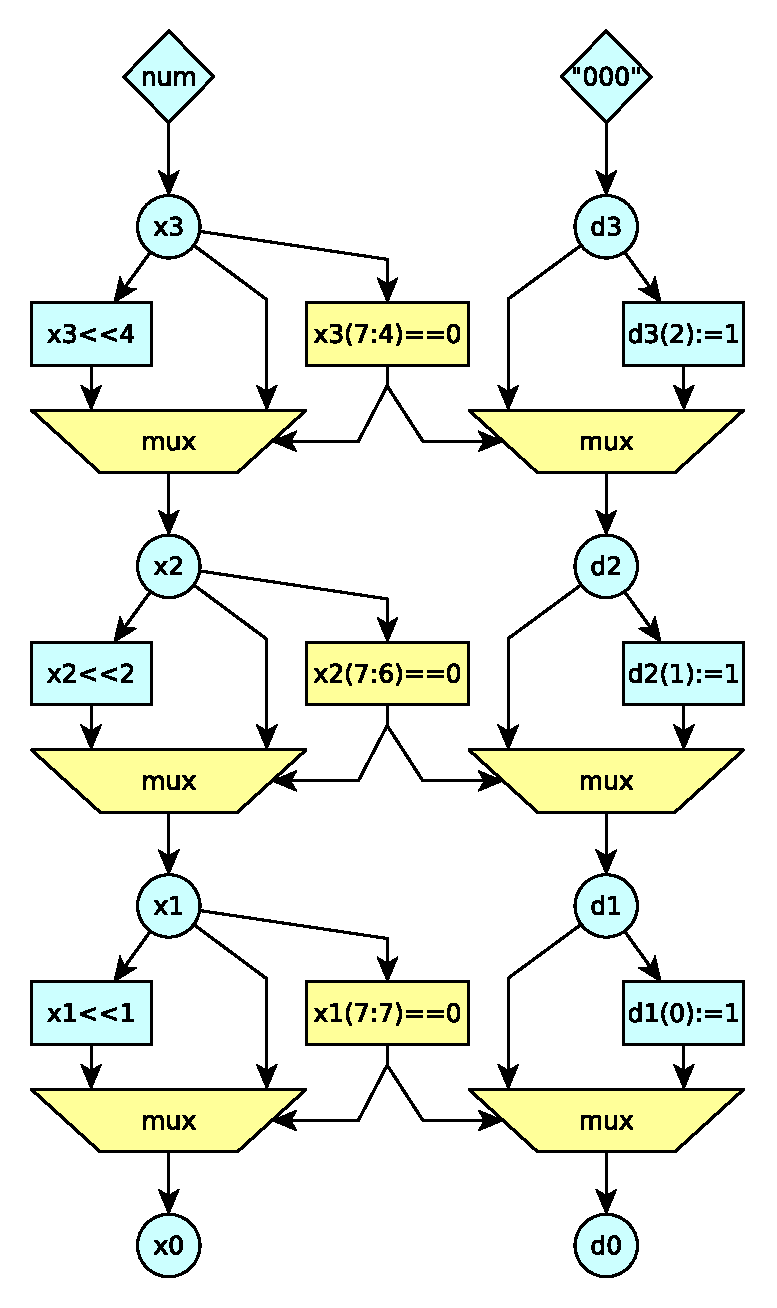
\includegraphics[width=0.8\linewidth]{graphics/lzc_dataflow.pdf}
  \captionof{figure}{Two steps dataflow example}
  \label{fig:LZC_Dataflow}
\end{figure}

%\setalgorithmicfont{\small}
%\begin{figure*}[h]
%  \centering
%  \begin{subfigure}[b]{0.32\textwidth}
%  \begin{algorithm}[H]
%    \caption*{Combined leading-zero counting and shifting}
%    \begin{algorithmic}
%      \fontsize{8}{8}\selectfont
%      \STATE{$k \leftarrow \left\lceil \log_2{n} \right\rceil$}
%      \STATE{$x_k \leftarrow x$}
%      
%      \FOR{$i = k-1$ downto $0$}
%      \IF{there are $2^i$ leading zeros in $x_{i+1}$} 
%      \STATE{$d_i \leftarrow 1$}
%      \STATE{$x_i \leftarrow x_{i+1}$, shifted left by $2^i$}
%      \ELSE 
%      \STATE{$d_i \leftarrow 0$}
%      \STATE{$x_i \leftarrow x_{i+1}$}
%      \ENDIF
%      \ENDFOR
%      \STATE{return $(d, x0)$}
%    \end{algorithmic}
%  \end{algorithm}
%  \caption{Pseudo code reference}
%  \end{subfigure}
%  \hfill
%  \begin{subfigure}[b]{0.32\textwidth}
%    \begin{minted}[autogobble,tabsize=2,fontsize=\fontsize{8}{8}\selectfont]{Scala}
%      def lzc_shift[N](num : DFBits[N]) = {
%        val k = log2Up(num.width)
%        val x = DFBits(num.width) := num
%        val d = DFBits(k) := 0
%        
%        for (i <- k-1 downto 0) {
%          ifdf (x.msbits(2~^i) == 0) {
%            d(i) := 1
%            x := x << 2~^i
%          }
%        }
%        (d, x)
%      }
%    \end{minted}
%    \caption{DFiant Code}
%  \end{subfigure}
%  \hfill
%  \begin{subfigure}[b]{0.32\textwidth}
%    \begin{minted}[autogobble,tabsize=2,fontsize=\fontsize{8}{8}\selectfont]{Scala}
%      //@ num : DFBits[8]
%      val x_3 = DFBits[8] := num
%      val d_3 = DFBits[3] := 0
%      val x_2 = mux(x_3.msbits(4)==0, x_3<<4, x_3)
%      val d_2 = mux(x_3.msbits(4)==0, d_3(2):=1, d_3)
%      val x_1 = mux(x_2.msbits(2)==0, x_2<<2, x_2)
%      val d_1 = mux(x_2.msbits(2)==0, d_2(1):=1, d_2)
%      val x_0 = mux(x_1.msbits(1)==0, x_1<<1, x_1)
%      val d_0 = mux(x_1.msbits(1)==0, d_1(0):=1, d_1)
%      (d_0, x_0)
%    \end{minted}
%    \caption{Unrolled Code}
%  \end{subfigure}
%  \caption{LZC+Shift code example}\label{fig:LZC+Shift code example}
%\end{figure*}

